\documentclass{article}
\usepackage[utf8]{inputenc}
\usepackage{fancyhdr}

\pagestyle{fancy}
\fancyhf{}
\rhead{PLP}
\lhead{Pràctica de Haskell}
\rfoot{ \thepage}
\lfoot{ }

\title{Paradigmes i Llenguatges de Programació\\ [Pràctica de Haskell]\\ $[$Verificador d'escacs$]$}
\author{Robert Ripoll & David Suárez}
\date{May 2019}
\usepackage{hyperref}
\usepackage{lipsum}
\usepackage[sort, numbers]{natbib}
\usepackage[table,xcdraw]{xcolor}
\usepackage{graphicx}
\usepackage{xcolor}
\usepackage{tcolorbox}
\usepackage{listings}
\usepackage{caption}
\DeclareCaptionFont{white}{\color{white}}
\DeclareCaptionFormat{listing}{%
  \parbox{\textwidth}{\colorbox{gray}{\parbox{\textwidth}{#1#2#3}}\vskip-4pt}}
\captionsetup[lstlisting]{format=listing,labelfont=white,textfont=white}
\lstset{frame=lrb,xleftmargin=\fboxsep,xrightmargin=-\fboxsep}

\begin{document}
\maketitle
\begin{figure}[h!]
\centering
\includegraphics[scale=0.35]{queen2.png}}
\begin{center}\textit{Be aware, she can move in any direction.}\end{center}
\end{figure}
\newpage
\tableofcontents

\newpage
\section{Introducció i objectius}
Partint de l'enunciat: \\
Es demana que feu un programa interactiu amb Haskell on es demani a l’usuari el nom del fitxer on hi hagi la partida en notació algebraica estesa per a analitzar i el programa vagi representant textualment la situació de la partida, tirada a tirada, fins al final $[$...$]$.
\\[0.2cm]
Hem desenvolupat un petit programa en Haskell que ens permet llegir fitxers de partides o conjunt de jugades d'escacs, tot seguint la notació algebraica especificada al document \textit{escacs.pdf} de l'enunciat de la pràctica.
\\[0.2cm] Si bé tot els recursos que hem fet servir, formen part del propi GHCI, hem hagut d'explicitar les següents exportacions de \textif{Data}:\\
\begin{tcolorbox}
import Data.Char\\
import Data.Maybe
\end{tcolorbox}
\noindent
La sortida del nostre programa, és una representació ASCII d'un tauler d'escacs. D'altra banda, totes les partides han de partir de l'escenari inicial d'un tauler d'escacs, tal com representem a continuacio:\\
\begin{figure}[ht!]
\centering
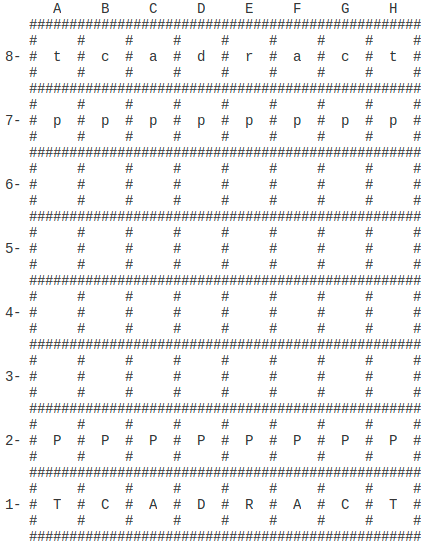
\includegraphics[scale=0.44]{board.png}}
\begin{center}Representació ASCII d'un tauler d'escacs\end{center}
\end{figure}
\newpage
\section{Exemples d'execució}
\subsection{Exemple: Pastor}
En aquest exemple, utilitzarem el fitxer d'entrada donat pel professor \textit{pastor.txt} on es realitza la coneguda jugada, per part de les peces Blanques. La partida no conté cap error, i pertant, acaba correctament:\\
\begin{tcolorbox}
llegirPartida "pastor.txt"
\end{tcolorbox}
\begin{tcolorbox}
Ronda 1.
Blanques: Jugada 'P' 'e'2 'e'4
Negres:   Jugada 'p' 'e'7 'e'5
Ronda 2.
Blanques: Jugada 'A' 'f'1 'c'4
Negres:   Jugada 'c' 'b'8 'c'6
Ronda 3.
Blanques: Jugada 'D' 'd'1 'h'5
Negres:   Jugada 'c' 'g'8 'f'6
Ronda 4. 
Blanques: EscacMat 'D' 'h'5 'f'7
Negres:   No juguen
\end{tcolorbox}
\begin{figure}[ht!]
\centering
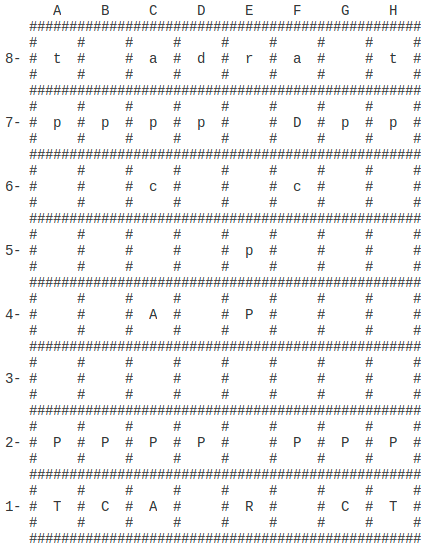
\includegraphics[scale=0.45]{pastor.png}}
\begin{center}Configuració final en \textit{pastor.txt}\end{center}
\end{figure}

\subsection{Exemple: Pastor \textbf{amb error}}
En aquest exemple, fem servir un fitxer \textit{pastor\_error.txt} on es realitza la coneguda jugada, per part de les peces Blanques. No obstant, hem determinat un error en la descripció de les jugades, i és que el darrer moviment de les blanques, malgrat ser Escac Mat, s'indica només l'escac. És a dir Dh5xf7+ en lloc de Dh5xf7++ :\\
\begin{tcolorbox}
llegirPartida "pastor\_error.txt"
\end{tcolorbox}
\begin{tcolorbox}
Ronda 1.
Blanques: Jugada 'P' 'e'2 'e'4
Negres:   Jugada 'p' 'e'7 'e'5
Ronda 2.
Blanques: Jugada 'A' 'f'1 'c'4
Negres:   Jugada 'c' 'b'8 'c'6
Ronda 3.
Blanques: Jugada 'D' 'd'1 'h'5
Negres:   Jugada 'c' 'g'8 'f'6
Ronda 4.
Blanques: Escac 'D' 'h'5 'f'7
Negres: No juguen

INVALID: Ronda 4. Jugador amb peces Blanc: S'ha indicat ESCAC, i és MAT
\end{tcolorbox}

\subsection{Exemple: Prova \textbf{amb error}}
En aquest exemple, fem servir un fitxer \textit{prova.txt} on es realitza senzillament un moviment impossible de la Dama Blanca, partint de la disposició inical del tauler, la volem situar a H5, pertant Dd1h5.
\begin{tcolorbox}
llegirPartida "prova.txt"
\end{tcolorbox}
\begin{tcolorbox}
Ronda 1.
Blanques: Jugada 'D' 'd'1 'h'5
Negres:  No juguen

INVALID: Ronda 1. Jugador amb peces Blanc: Hi ha una peça pel mig entre la posició origen i la posició destí la jugada.
\end{tcolorbox}
\newpage
\subsection{Exemple: Partida inmortal}

En aquest exemple, fem servir el fitxer \textit{partida\_inmortal.txt} donat amb la pràctica, la partida acaba amb la victoria per part de les peces Blanques. És una partida amb 23 rondes que transcorren amb normalitat:\\
\begin{tcolorbox}
llegirPartida "partida\_inmortal.txt"
\end{tcolorbox}
\begin{tcolorbox}
Ronda 1.
Blanques: Jugada 'P' 'e'2 'e'4
Negres:   Jugada 'p' 'e'7 'e'5
Ronda 2.
Blanques: Jugada 'P' 'f'2 'f'4
Negres:   Captura 'p' 'e'5 'f'4
Ronda 3.
Blanques: Jugada 'A' 'f'1 'c'4
Negres:   Escac 'd' 'd'8 'h'4
Ronda 4.
Blanques: Jugada 'R' 'e'1 'f'1
Negres:   Jugada 'p' 'b'7 'b'5
Ronda 5.
Blanques: Captura 'A' 'c'4 'b'5
Negres:   Jugada 'c' 'g'8 'f'6
Ronda 6.
Blanques: Jugada 'C' 'g'1 'f'3
Negres:   Jugada 'd' 'h'4 'h'6
Ronda 7.
Blanques: Jugada 'P' 'd'2 'd'3
Negres:   Jugada 'c' 'f'6 'h'5
Ronda 8.
Blanques: Jugada 'C' 'f'3 'h'4
Negres:   Jugada 'd' 'h'6 'g'5
Ronda 9.
Blanques: Jugada 'C' 'h'4 'f'5
Negres:   Jugada 'p' 'c'7 'c'6
Ronda 10.
Blanques: Jugada 'P' 'g'2 'g'4
Negres:   Jugada 'c' 'h'5 'f'6
Ronda 11.
Blanques: Jugada 'T' 'h'1 'g'1
Negres:   Captura 'p' 'c'6 'b'5
Ronda 12.
Blanques: Jugada 'P' 'h'2 'h'4
Negres:   Jugada 'd' 'g'5 'g'6
Ronda 13.
Blanques: Jugada 'P' 'h'4 'h'5
Negres:   Jugada 'd' 'g'6 'g'5
Ronda 14.
Blanques: Jugada 'D' 'd'1 'f'3
Negres:   Jugada 'c' 'f'6 'g'8
Ronda 15.
Blanques: Captura 'A' 'c'1 'f'4
Negres:   Jugada 'd' 'g'5 'f'6
Ronda 16.
Blanques: Jugada 'C' 'b'1 'c'3
Negres:   Jugada 'a' 'f'8 'c'5
Ronda 17.
Blanques: Jugada 'C' 'c'3 'd'5
Negres:   Captura 'd' 'f'6 'b'2
Ronda 18.
Blanques: Jugada 'A' 'f'4 'd'6
Negres:   Captura 'a' 'c'5 'g'1
Ronda 19.
Blanques: Jugada 'P' 'e'4 'e'5
Negres:   Escac 'd' 'b'2 'a'1
Ronda 20.
Blanques: Jugada 'R' 'f'1 'e'2
Negres:   Jugada 'c' 'b'8 'a'6
Ronda 21.
Blanques: Escac 'C' 'f'5 'g'7
Negres:   Jugada 'r' 'e'8 'd'8
Ronda 22.
Blanques: Escac 'D' 'f'3 'f'6
Negres:   Captura 'c' 'g'8 'f'6
Ronda 23.
Blanques: EscacMat 'A' 'd'6 'e'7
Negres:  No juguen
\end{tcolorbox}
\begin{figure}[ht]
\centering
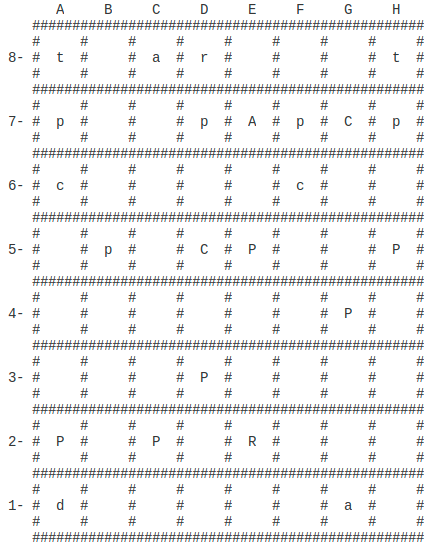
\includegraphics[scale=0.45]{partida_inmortal.png}
\begin{center}Configuració final en \textit{partida\_inmortal.txt}\end{center}
\end{figure}
\noindent
\newpage
\subsection{Exemple: Rei destapat \textbf{amb error}}
En aquest exemple, fem servir el fitxer \textit{rei\_destapat.txt} on ens trobem en la situació on les peces Blanques intenten realitzar un moviment amb el Peó situat a G3, que destaparien el rei i el posarien en Escac:
\begin{tcolorbox}
llegirPartida "rei\_destapat.txt"
\end{tcolorbox}
\begin{tcolorbox}
Ronda 1.
Blanques: Jugada 'P' 'e'2 'e'4
Negres:   Jugada 'p' 'e'7 'e'5
Ronda 2.
Blanques: Jugada 'P' 'f'2 'f'4
Negres:   Captura 'p' 'e'5 'f'4
Ronda 3.
Blanques: Jugada 'A' 'f'1 'c'4
Negres:   Escac 'd' 'd'8 'h'4
 Ronda 4.
Blanques: Jugada 'P' 'g'2 'g'3
Negres:   Jugada 'p' 'b'7 'b'5
Ronda 5.
Blanques: Jugada 'P' 'g'3 'g'4
Negres:   Captura 'd' 'h'4 'g'4

INVALID: Ronda 5. Jugador amb peces Blanc: La situació actual és d'escac, i la jugada segueix en escac.
\end{tcolorbox}

\newpage
\subsection{Exemple: Escac eliminat \textbf{amb error}}

En aquest exemple, fem servir el fitxer \textit{escac\_eliminat.txt} on ens trobem amb un moviment invàlid del Peó Negre que es troba a F4, quan s'indica a la partida que realitza una \textbf{captura}. Imaginem que la partida està mal representada, i es volía fer la jugada Pf4xg3. No obstant, sent fidels al fitxer, tenim la següent partida:
\begin{tcolorbox}
llegirPartida "escac\_eliminat.txt"
\end{tcolorbox}
\begin{tcolorbox}
Ronda 1.
Blanques: Jugada 'P' 'e'2 'e'4
Negres:   Jugada 'p' 'e'7 'e'5
Ronda 2.
Blanques: Jugada 'P' 'f'2 'f'4
Negres:   Captura 'p' 'e'5 'f'4
Ronda 3.
Blanques: Jugada 'A' 'f'1 'c'4
Negres:   Escac 'd' 'd'8 'h'4
Ronda 4.
Blanques: Jugada 'P' 'g'2 'g'3
Negres:   Escac 'd' 'h'4 'g'3
Ronda 5.
Blanques: Captura 'P' 'h'2 'g'3
Negres:   Captura 'p' 'f'4 'f'3

INVALID: Ronda 5. Jugador amb peces Negre: S'ha indicat CAPTURA, i no ho és.
\end{tcolorbox}

\subsection{Exemple: Escac no resolt \textbf{amb error}}

En aquest exemple, fem servir el fitxer \textit{escac\_no\_resolt.txt} on ens trobem amb el Rei Negre que es troba en Escac i el moviment que preten fer per ensortir-se'n, és invàlid pel multiples raons. En primer lloc, continuaria estant en Escac, i daltra banda també hi ha un Peó Negre a F2.
\begin{tcolorbox}
llegirPartida "error\_escac\_no\_resolt.txt"
\end{tcolorbox}
\begin{tcolorbox}
Ronda 1.
Blanques: Jugada 'P' 'e'2 'e'4
Negres:   Jugada 'p' 'e'7 'e'5
Ronda 2.
Blanques: Jugada 'P' 'f'2 'f'4
Negres:   Captura 'p' 'e'5 'f'4
Ronda 3.
Blanques: Jugada 'A' 'f'1 'c'4
Negres:   Escac 'd' 'd'8 'h'4
Ronda 4.
Blanques: Jugada 'R' 'e'1 'f'2
Negres:   Jugada 'p' 'b'7 'b'5

INVALID: Ronda 4. Jugador amb peces Blanc: La situació actual és d'escac, i la jugada segueix en escac.
\end{tcolorbox}
\newpage
\subsection{Exemple: Enroc llarg}

En aquest exemple, fem servir el fitxer \textit{enroc\_llarg.txt} on fem una partida simètrica pel que fa als moviments dels dos colors, possiblititant que tots dos facin l'enroc llarg.
\begin{tcolorbox}
llegirPartida "enroc\_llarg.txt"
\end{tcolorbox}
\begin{tcolorbox}
Ronda 1.
Blanques: Jugada 'P' 'd'2 'd'4
Negres:   Jugada 'p' 'd'7 'd'5
Ronda 2.
Blanques: Jugada 'A' 'c'1 'e'3
Negres:   Jugada 'a' 'c'8 'e'6
Ronda 3.
Blanques: Jugada 'C' 'b'1 'a'3
Negres:   Jugada 'c' 'b'8 'a'6
Ronda 4.
Blanques: Jugada 'D' 'd'1 'd'2
Negres:   Jugada 'd' 'd'8 'd'7
Ronda 5.
Blanques: EnrocLlarg 
Negres: EnrocLlarg  
\end{tcolorbox}
\begin{figure}[ht]
\centering
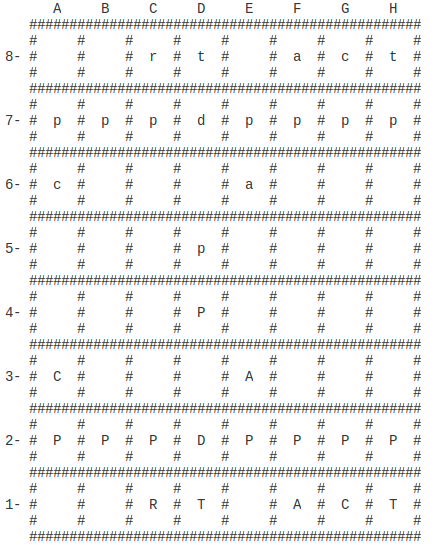
\includegraphics[scale=0.45]{enroc.png}
\begin{center}Configuració final en \textit{enroc\_llarg.txt}\end{center}
\end{figure}

\newpage
\section{Codi font i funcions}
\subsection{Tipus de dades}
\begin{itemize}
    \item data Color = Blanc $|$ Negre deriving (Eq, Show)
    \item data TipusPeca = Rei $|$ Reina $|$ Torre $|$ Alfil $|$ Cavall $|$ Peo deriving Eq
    \item data Peca = Pec TipusPeca Color deriving Eq
    \item data Tauler = Tau [(Posicio, Peca)]
    \item data Posicio = Char :/ Int deriving Eq
    \item data JugadaGenerica = Jugada Peca Posicio Posicio $|$ Captura Peca Posicio Posicio $|$ EnrocCurt Peca Posicio Posicio $|$ EnrocLlarg Peca Posicio Posicio $|$ Escac Peca Posicio Posicio $|$ EscacMat Peca Posicio Posicio deriving (Eq, Show)
    \item data Jugada = Jug Peca Posicio Posicio deriving Eq
    \item type Casella = (Posicio, Peca)
    \item data Partida = Par Tauler Color (Actualment no utilitzada)
\end{itemize}
\subsection{Moviments}
\subsubsection*{posicioUp :: Posicio -$>$ Posicio}
Retorna el desplaçament d'una posició més adalt respecte la posició passada per paràmetre.
\subsubsection*{posicioDown :: Posicio -$>$ Posicio}
Retorna el desplaçament d'una posició més adalt respecte la posició passada per paràmetre.
\subsubsection*{posicioRight :: Posicio -$>$ Posicio}
Retorna el desplaçament d'una posició més a la dreta respecte la posició passada per paràmetre.
\subsubsection*{posicioLeft :: Posicio -$>$ Posicio}
Retorna el desplaçament d'una posició més a l'esquerra respecte la posició passada per paràmetre.
\subsubsection*{posicioDiagSupEsq :: Posicio -$>$ Posicio}
Retorna el desplaçament d'una posició més a la diagonal superior esquerra respecte la posició passada per paràmetre.
\subsubsection*{posicioDiagSupDreta :: Posicio -$>$ Posicio}
Retorna el desplaçament d'una posició més a la diagonal superior dreta respecte la posició passada per paràmetre.
\subsubsection*{posicioDiagInfEsq :: Posicio -$>$ Posicio}
Retorna el desplaçament d'una posició més a la diagonal inferior esquerra respecte la posició passada per paràmetre.
\subsubsection*{posicioDiagInfDreta :: Posicio -$>$ Posicio}
Retorna el desplaçament d'una posició més a la diagonal inferior dreta respecte la posició passada per paràmetre.

\subsection{Mètodes rellevants}
\subsection*{trobarPeca :: Tauler -$>$ Posicio -$>$ Maybe Peca}
Retorna la peça ("Just Peça") del tauler passat per paràmetre
que es troba a la posició passada per paràmetre. Si la posició
no existeix retorna "Nothing".
\subsection*{trobarPeces :: Tauler -$>$ [Posicio] -$>$ [Maybe Peca]}
Retorna un conjunt de peces que tenen la posició passada per
paràmetre en una llista, d'acord amb el tauler passat per
paràmetre. Si una posició de les passades a la llista no es
troba, s'afegirà un "Nothing" a la llista a retornar; en cas
que es trobi, s'afegirà un "Just Peca".
\subsection*{aplicarFunc :: (Posicio -$>$ Posicio) -$>$ Posicio -$>$ [Posicio]}
Aplica una funció passada per paràmetre a una posició
passada per paràmetre, i retorna, en un llistat, el resultat
d'aplicar la funció a la posició, de tornar a aplicar la funció
al previ resultat i així successivament fins trobar una
posició no vàlida.
\subsection*{generarMoviments :: Peca -$>$ Posicio -$>$ [Posicio]}
Genera les posicions on pot anar una peça passada per
paràmetre trobant-se en una posició passada per paràmetre,
d'acord amb les regles del joc i com es pot moure la peça.
\subsection*{generarPosicions :: Posicio -$>$ Posicio -$>$ (Posicio -$>$ Posicio) -$>$ [Posicio]}
Retorna les posicions dins d'un interval passat per paràmetre
(posA, posB) aplicant una funció passada per paràmetre fins
trobar una posició no vàlida o que sigui la posició B.
Dins d'aquesta llista de posicions s'exclouen tant posA com posB.
\subsection*{posicionsEntre :: Posicio -$>$ Posicio -$>$ [Posicio]}
Retorna les posicions que es troben dins de l'interval passat
per paràmetre (posA, posB). Dins d'aquesta llista de posicions
s'exclouen tant posA com posB.
\subsection*{alguEntre :: Tauler -$>$ Posicio -$>$ Posicio -$>$ Bool}
Retorna cert si hi ha alguna peça entre dues posicions
passades per paràmetre (excloent les dues posicions, es clar);
fals altrament.
\subsection*{aplicarJugada :: Tauler -$>$ Jugada -$>$ Bool -$>$ [(Posicio, Peca)]}
Retorna el resultat d'aplicar una jugada passada per paràmetre
sobre el tauler passat per paràmetre. El booleà passat per paràmetre
indica si s'ha trobat la casella de la posició destí de la jugada o no.
\subsection*{fesJugada :: Tauler -$>$ Jugada -$>$ Tauler}
Retorna un nou tauler resultant d'aplicar la jugada passada per
paràmetre, partint del tauler (estat actual del joc) passat per
paràmetre.
\subsection*{trobarRei :: Tauler -$>$ Color -$>$ Posicio}
Retorna la posició del rei del bàndol del color passat per paràmetre
d'acord amb el tauler passat per paràmetre.
\subsection*{jugadesColor :: Tauler -$>$ Color -$>$ [Jugada]}
A partir de l'estat actual de la partida (el tauler passat per paràmetre)
i un bàndol (color passat per paràmetre), retorna les possibles jugades
vàlides i legals que pot fer.
\subsection*{movimentsColor :: Tauler -$>$ Color -$>$ [Posicio]}
Retorna un llistat amb els moviments que poden fer les peces del
bàndol del color passat per paràmetre d'acord amb el tauler passat
per paràmetre.
\subsection*{escac :: Tauler -$>$ Color -$>$ Bool}
Retorna cert si el bàndol del color passat per paràmetre està en escac
a l'estat actual de la partida (el tauler passat per paràmetre); retorna
fals altrament.
\subsection*{jugadaValida :: Tauler -$>$ Jugada -$>$ Int}
Si la jugada és vàlida, retornarà 0 o 1. Això es determinarà a partir de
la jugada que es vol fer i l'estat del tauler, que són elements que es passen
per paràmetre. Retornarà 0 quan la jugada passada sigui vàlida i no es capturi
a cap peça contrincant. Si la jugada és vàlida però es captura una peça contrincant,
es retornarà 1. Si la jugada no és vàlida, retorna:
\begin{itemize}
 \item-1 -$>$ "La casella origen de la jugada esta buida"
 \item-2 -$>$ "La peça de la casella origen no coincideix amb la peça de la jugada"
 \item-3 -$>$ "El moviment de la jugada no és vàlid d'acord amb els moviments que pot fer la peça"
  \item-4 -$>$ "Hi ha una peça pel mig entre la posició origen i la posició destí la jugada"
 \item-5 -$>$ "La posició destí de la jugada està ocupada per una peça del mateix jugador que fa la jugada"
   \item-6 -$>$ "La situació actual és d'escac, i la jugada segueix en escac"
\end{itemize}
\subsection*{escacMat :: Tauler -$>$ Color -$>$ Bool}
Retorna cert si el bàndol amb el color passat per paràmetre està en escac mat;
retorna fals altrament.
\subsection*{llegirLinia :: String -$>$ (String, JugadaGenerica, Maybe JugadaGenerica)}
Llegeix una linia del tipus "1. Pe2e4 Pe7e5" i ho parseja
en forma de Tupla, tenint en compte si son 2 o 3 paràmetres.
\subsection*{llegirJugada :: String -$>$ Color -$>$ JugadaGenerica}
Donat un String com per exemple "Pe7e5" o "Dh5xf7++" o "0-0" 
retorna el tipus de JugadaGenerica concret que és.
\subsection*{tractaUnaJugada :: String -$>$ Tauler -$>$ Color -$>$ JugadaGenerica -$>$ Tauler}
Des d'aquesta funció es controlen els errors d'invalidesa d'una 
determinada jugada. Tanmateix és la que a partir de subtipus de
JugadaGenerica donat, i el tauler, s'efectuaran les comprovacions
i les crides a fesJugada.
\subsection*{evalua :: Tauler -$>$ (String, JugadaGenerica, Maybe JugadaGenerica) -$>$ Tauler}
Donat un Tauler i una tupla de tres elements, comprovem si
es tracta d'una jugada de blanques unicament o bé de ambdós
colors intervenint. Retorna el tauler havent aplicat les jugades. 
\subsection*{iteraRondes :: Tauler -$>$ [(String, JugadaGenerica, Maybe JugadaGenerica)] -$>$ IO()}
En aquesta funció es mostren els missatges de informació sobre 
les diferents Rondes, amb el respectiu tauler, etc. No només mostra,
sinó que recursivament crida a la funció evalua mentre mostra missatges.
\subsection*{llegirPartida :: String -$>$ IO()}
Exemple d'ús: llegirPartida "pastor.txt"
Interpreta la partida i la tradueix a Jugades, s'evaluen a "evalua"
\newpage
\section{Resultat i valoracions}
El resultat és un petit programa que contempla la majoría de casuístiques del joc. No obstant, quedaria pendent vàries de les millores proposades com pot ser detectar taules, etc.\\[0.2cm]
Pel que fa al paradigma de programació funcional, i concretament al Haskell la comprensió de funcions és més fàcil respecte la programació declarativa i imperativa ja que les funcions estan escrites a un molt alt nivell.\\El fet que Haskell sigui pur i garanteixi transparència referencial ens facilita el testing, ja que si una funció retorna un valor equivocat només haurem de traçar el fil i seguir els valors que són erronis, ignorant la resta de l'aplicació. Comparant aquest tipus de programació (la funcional) amb la programació tradicional imperativa, amb la programació funcional estàs descrivint el que vols en comptes de com ho vols.
\begin{thebibliography}{9}
\bibitem{ref1} 
\textbf{Pàgina de consulta}\\
\url{http://zvon.org/other/haskell/Outputglobal/index.html}

\bibitem{ref2}
\textbf{Pàgina de consulta}\\
\url{https://wiki.haskell.org/Haskell}

\end{thebibliography}


\end{document}
